\documentclass[12pt]{report}
\usepackage{hepnicenames}
\usepackage{subcaption}
\usepackage{graphicx}
\usepackage[T1]{fontenc}
\usepackage[utf8]{inputenc}
\usepackage{titlepic}
\usepackage{hyperref}
\usepackage{gensymb}
\usepackage{subfiles}
\usepackage{siunitx}
\usepackage{makecell}
\usepackage[a4paper, margin=2cm]{geometry}
\usepackage{fourier}
\usepackage{tabularx}
\usepackage{array}
\usepackage{caption}
\usepackage{amsmath}
\usepackage{commath}
\usepackage{amssymb}
\usepackage{makecell}

\renewcommand\theadalign{bc}
\renewcommand\theadfont{\bfseries}
\renewcommand\theadgape{\Gape[4pt]}
\renewcommand\cellgape{\Gape[4pt]}

\title{Cosmic muon magnetic moment and lifetime}
\author{Matei A.V. Climescu}
\date{Mainz,2020}

\newenvironment{changemargin}[2]{%
\begin{list}{}{%
\setlength{\topsep}{0pt}%
\setlength{\leftmargin}{#1}%
\setlength{\rightmargin}{#2}%
\setlength{\listparindent}{\parindent}%
\setlength{\itemindent}{\parindent}%
\setlength{\parsep}{\parskip}%
}%
\item[]}{\end{list}}




\begin{document}
\maketitle

\begin{titlepage}
\begin{changemargin}{-0cm}{-0cm}
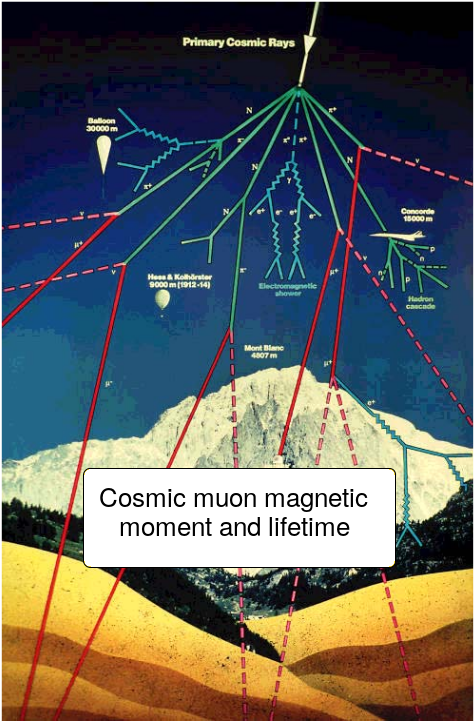
\includegraphics[width=\linewidth]{./fig/cover.png}
\end{changemargin}
\end{titlepage}



    
\chapter{Introduction}

This experiment is based on the Diplomarbeit of Mathias Heel in 1982 (\textit{Aufbau eines Versuchs im Fortgeschrittenen-Praktikum zur Messung der Lebendauer von Myonen}) and in particular the Staatsexamensarbeit of Joachim Geisb\"{u}sch in 1991 (Verbesserungen zum Experiment) at the University of Mainz's Departement of Physics. This experiment script was re-written in English by Matei Climescu in 2020 from Andreas Winhart's German version from 2001. The full script is available at \href{https://github.com/matclim/muonlifetime} and is publicly available for improvements, updates and changes there.



This experiment allows for the determination of the lifetime and magnetic moment of cosmic muons. Students can have a first introduction to elementary particle physics measurements and analysis methods with relatively simple means. 


The muon \Pmuon is an elementary particle often referred to as the electron's `heavy cousin'. It has identical properties to the electron and thus behaves in the same way, if the electron's mass was 207 times larger. The same can be said for the charged tau lepton \Ptauon (sometimes called the tauon) albeit with a 3491 mass factor instead. This gives rise to the concept of Lepton universality. The reason why the number of lepton generations is three remains unclear. Muons are of particular interest because:


\begin{itemize}
\item Parity violation in the weak sector is a particularly important part of modern physics: nature isn't invariant to spatial transformations, this is one of the results of the experiment.

\item A fairly accurate measurement for the weak coupling constant can be performed along with the muon's lifetime. The measurement of the anomalous magnetic moment of the muon, the so-called `g-2 factor' is an important test for the validity of QED.

\item Muons are the main component of sea-level cosmic radiation. The radiation density remains low however: the verticle flux of muons above \SI{1}{GeV/c}
\end{itemize}


    % !TEX root = Experiment41.tex

 
 \chapter{The Standard Model of Particle Physics}
 
 
 
After closer investigation of cosmic radiation, many new particles were discovered, such as neutral Kaons \PKzero in 1947, prompting Nobel prize Willis Lamb to declare ``The finder of a new elementary particle used to be rewarded by a Nobel Prize, but such a discovery now ought to be punished by a 10,000 dollar fine.''. As new techniques, such as particle accelerators, were improved, this `Particle Zoo' became more and more confusing to physicists. In the 1960s and 70s, a new model emerged: the Standard Model which brought order to the apparent chaos. It did so by articulating the phenomenology of known fundamental interactions into a single self-consistent, locally gauge-invariant quantum field theory centered around electromagnetism (Quantum Electro-Dynamics or \textit{QED}), the strong nuclear force (Quantum Chromo-Dynamics or \textit{QCD}) and the weak nuclear force.

Those interactions are mediated by spin-1 particles, the so called \textit{vector-bosons}: the photon \Pgamma mediates QED, eight massless but coloured gluons \Pgluon mediate QCD and three massive bosons \PZ, \PWpm mediate the weak interaction. Finally a single spinless massive \textit{scalar boson}, the so called \textit{Higgs Boson} was observed in 2012 and allows for massive bosons and at least certain fermions to be massive. All those bosons can be found in Table \ref{tab:bosons}. Each interaction takes place via the exchange of its bosons, for example, the $\beta^{-}$-decay of $^{137}\text{Cs}$ to $^{137}\text{Ba}$ can in fact be seen as a neutron's \Pdown emitting a \PWminus and thus becoming a \Pup, causing the neutron to become a proton. This reaction can be seen in Figure \ref{fig:betadecay}.
Matter however is made of fermions, particle with spin $\frac{1}{2}$, those, in the Standard Model are classified as \textit{quarks} and \textit{leptons}.
The Standard Model was observed to hold  6 massive quarks, reacting to all three interactions, 3 charged leptons, sensitive to electromagnetism and the weak interaction, and 3 neutral leptons, \textit{neutrinos}, which only interact through the weak interaction. They can be found in Table \ref{tab:SM}.

\begin{table}[htbp]
\centering
\resizebox{\linewidth}{!}{%
\begin{tabular}{|c|c|c|c|c|c|c|}
\hline
\textbf{Generation} & \multicolumn{2}{c|}{\textbf{1}} & \multicolumn{2}{c|}{\textbf{2}} & \multicolumn{2}{c|}{\textbf{3}} \\ \hline
& Fermion & Mass [MeV] & Fermion & Mass [MeV] & Fermion & Mass [MeV] \\ \hline
Up-type quarks ($q=\frac{2}{3}$) & up (\Pup) & $\sim 2.2$ & charm (\Pcharm) & $\sim 1300$ & top (\Ptop) & $173000 $  \\ \hline
Down-type quarks ($q=\frac{+2}{3}$) & down (\Pdown) & $\sim 4.7$ & strange (\Pstrange) & $\sim 95$ & beauty/bottom (\Pbottom) & $\sim 4200$ \\ \hline
Charged leptons ($q=\frac{-1}{2}$) & electron (\Pelectron) & $0.511$  & muon (\Pmuon) & $113$ & tau (\Ptauon) & $1780$  \\ \hline
Neutrinos ($q=0$) &  electron neutrino (\Pnue) & $\sim 0$ & muon neutrino (\Pnum) & $\sim 0$ & tau neutrino (\Pnut) & 0 \\ \hline
\end{tabular}}
\caption{Standard Model fermions.}
\label{tab:SM}
\end{table}

\begin{table}[htbp]
\centering
\scriptsize
\setlength\tabcolsep{2pt}
\begin{tabular}{|c|c|c|c|c|c|c|c|}
\hline
\textbf{Interaction} & \textbf{Boson} & \textbf{Mass [GeV]} & \textbf{Range [m]} & \textbf{Time scale [s]} & \textbf{spin} & \textbf{coupling} & \textbf{Fields} \\ \hline
Strong & gluon (\Pgluon)& 0 & $10^{-15}$ & $10^{-23}$ & 1 & $\sim 1$ & Quarks \\ \hline
Electromagnetic & photon (\Pgamma) & 0 & $\inf$ & $10^{-20}$ & 1 & $1/137$ & Electric charge \\ \hline
Weak & Z-zero boson (\PZzero), W bosons (\PWpm) & 91.2, 80.4 &  $\sim 10^{-17}$ & $10^{-8}$ & 1 & $10^{-5}$ & Quarks and leptons \\ \hline
Higgs & boson \PHiggs & $ 125.2$ & $\sim 10^{-18}$ &  $\sim 10^{-22}$ & 0 & variable & Massive fields \\ \hline
Gravity & graviton ($g$) & 0 & $\inf$ & - & 2 & $> 10^{-41}$ & Massive fields \\ \hline

\end{tabular}
\caption{Standard Model force carriers.}
\label{tab:bosons}
\end{table}


\begin{figure}[htbp]
\centering
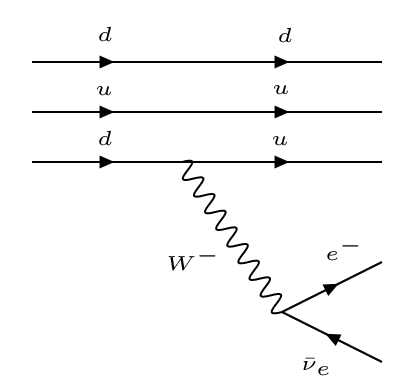
\includegraphics[width=0.5\linewidth]{./fig/betadecay.png}
\caption{Weak decay of a neutron to a proton.}
\label{fig:betadecay}
\end{figure}

Ordinary matter is overwhelmingly composed of first generation particles: \textit{up} and \textit{down}- type quarks and \textit{electrons}, a proton is notably composed of two up-type quarks and one down-type quark while a neutron is composed of a single up-type quark and two down-type quarks. It should be noticed that this is mostly due to the unstable nature of particles from Generation 2 and 3 (with the notable exception of neutrinos). Those particles will decay into lighter ones, it should be noted that, as a general rule, heavier particles decay faster and thus have a shorter lifetime. 


    
\chapter{Cosmic Radiation}

\section{History of cosmic radiation}

In 1785, Charles-Augustin de Coulomb discovered that charge was released by a charged electroscope over time. Over a century later, Wilson and Geitel discovered ionization currents using a bell apparatus shown in Figure \ref{fig:bell}. They noticed that a dark current persisted in the bell and that, despite it being weakened by covering the apparatus in lead, it could never quite be eliminated, leading them to postulate the existence of telluric radioactivity (or Earth radioactivity).

\begin{figure}[htbp]
\centering
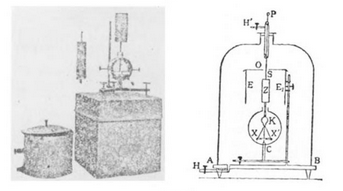
\includegraphics[width=0.6\linewidth]{./fig/bell.png}
\caption{Geitel's ionization current apparatus (1900).}
\label{fig:bell}
\end{figure}

It wasn't until 1912 that it was determined that the source of this ``dark current'' couldn't be the earth: Victor Hess experimented with putting an electroscope onto a balloon which he launched to an altitude of up to \SI{5300}{\meter}. He found that the rate of radiation was there some three times what it was at sea level and this, allied with his experimentation during a partial solar eclipse, allowed him to rule out the Sun as the source of this myterious radiation, enabling him to discover a natural source of high-energy particles: cosmic rays, awarding him the Nobel prize in 1936. Later studies from Freier, Lofgren, Ney, Oppenheimer, Bradt and Peters from 1948 and many others accross the years showed the existence of different radiation in the upper atmosphere, the so-called primary radiation, composed of around $90\%$ protons and around $10\%$ other nuclei which corresponds to the material ratio found in your average star, leading to the conclusion that cosmic radiation was mostly emitted by stars.

\section{Primary cosmic rays}

In star explosions, such as Supernovae, electric fields arise at the star's surface, this implies the acceleration of charged particles to very high energies. Particles thus gain enough energy to exit the star's potential well but whether they actually are able to be emitted is also dependent on their mass: lighter particles such as \Pelectron see their energy quickly depleted through \textit{bremsstrahlung emissions}. This is due to the way the emitted bremsstrahlung energy $E_\text{Brems}$ evolves relative to the emitting particle's mass $m_\text{P}$:

\begin{equation}
E_\text{Brems}	\propto \frac{1}{m_\text{P}^2}.
\end{equation}

This implies that protons and heavy nuclei are the main constituents of what exits the star.

When this primary radiation enters the atmosphere, it's deflected by the Earth's B-field via the Lorentz force. At our latitude (50\degree -Mainz Gutenbergplatz), particles require at least \SI{3}{\giga\electronvolt} to enter the atmosphere. This values varies around the globe and is in particular lower near the poles since there is a higher proportion of field lines parralel to the Earth's surface. This is often called the \textit{magnetic latitude effect} shown in Figure \ref{fig:magintensity}.


\begin{figure}[htbp]
\centering
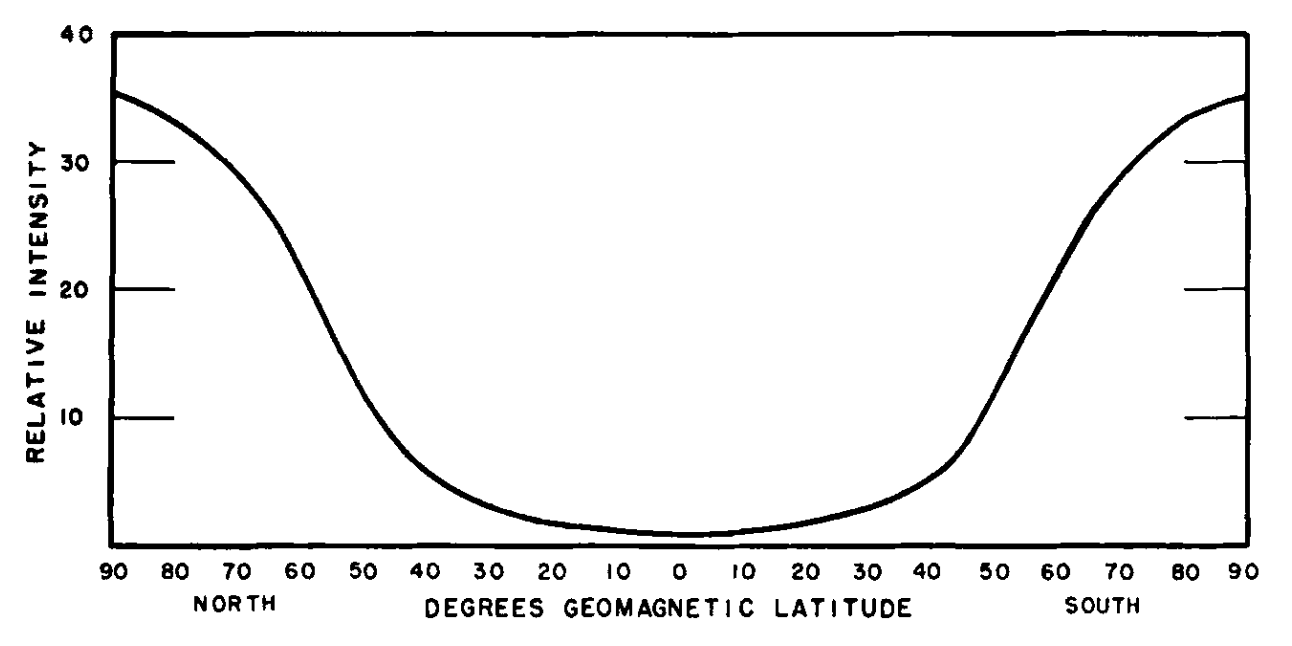
\includegraphics[width=0.8\linewidth]{./fig/intensity.png}
\caption{Magnetic latitude effect at sea level.}
\label{fig:magintensity}
\end{figure}

The Earth's $\mathbf{B}$-field is a dipole field with magnetic moment of $8.1 \cdot 10^{18}\text{ J}.\text{G}^{-1}$. The critical momentum, the minimal momentum needed to breach the atmosphere is given by:

\begin{equation}
\text{P}_\Phi=1.5\cdot 10^{10} \cos^4\Phi |z| \text{ eV}.c^{-1}.
\end{equation}

where $z$ is the particle's charge in units of elementary charge. The discrenpency in the number of positive and negative particles results in an east-west asymmetry in particle intensity. At least $90\%$ of the primary particles have a positive charge as shown in Figure \ref{fig:assym}.

\begin{figure}[htbp] %No better figure could be found, it could be remade%
\centering
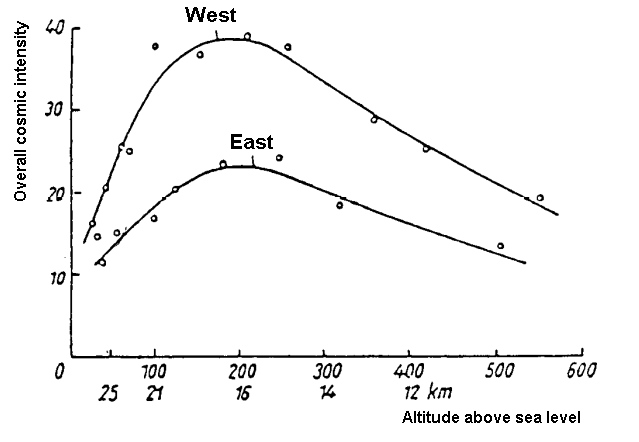
\includegraphics[width=0.8\linewidth]{./fig/assym.png}
\caption{East-west asymmetry measured at different altitudes.}
\label{fig:assym}
\end{figure}


\section{Secondary comic rays}

Since the atmosphere is a matter-rich environment, it provides any entering primary radiation with fields to interact with, which gives rise to a variety of processes, producing so-called \textit{secondary cosmic rays}. Low energy protons, with momenta up to \SI{10}{\giga\electronvolt} knock-off individual nucleons from nitrogen and oxygen nuclei. At higher energy, nuclear (meson-dominated) bremsstrahlung radiation is the main source of energy loss. An example of it can be found in Figure \ref{fig:scat}. 

\begin{figure}[htbp]
\centering
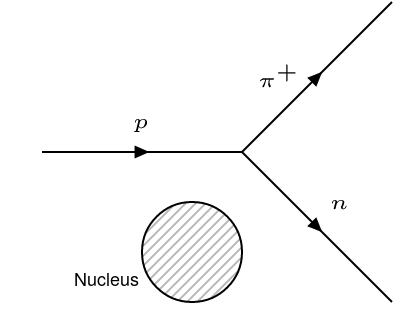
\includegraphics[width=0.5\linewidth]{./fig/nscat.png}
\caption{Bremsstrahlung pion emission from proton-nucleus scattering.}
\label{fig:scat}
\end{figure}






The produced mesons are mostly pions but heavier flavour particles can be created at energies above \SI{100}{\giga\electronvolt} such as Kaons.

Protons from primary cosmic rays have an energy up to a couple PeV and will thus also perform nucleon-antinucleon pairs. This energy level remains very rare however as can be seen in Figure \ref{fig:knee}

\begin{figure}[htbp]
\centering
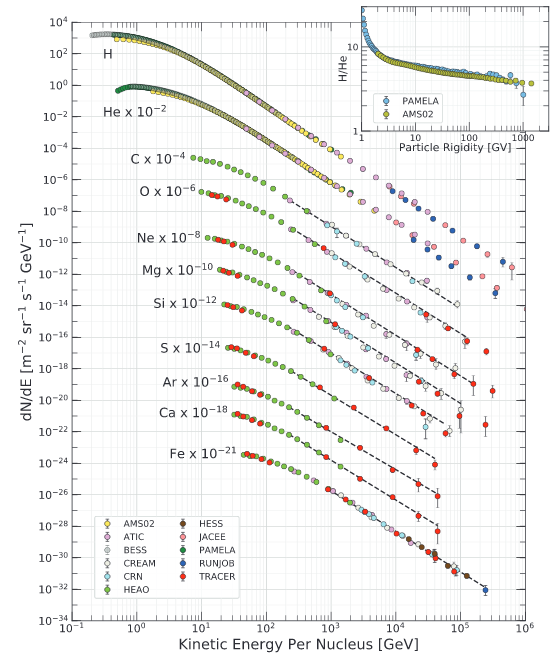
\includegraphics[width=\linewidth]{./fig/knee.png}
\caption{Fluxes of nuclei of the primary cosmic radiation in particles per-energy-per-nucleus are plotted vs energy-per-nucleus. The inset shows the H/He ratio at constant rigidity \cite{Tanabashi:2018oca}.}
\label{fig:knee}
\end{figure}

The number N of protons for a given energy is given by:

\begin{equation*}
\text{N}(E)=K\cdot E^{-\gamma}.
\end{equation*}

where $K$ is a constant and $\gamma$ varies with the energy: from $\gamma=1$ for $E=\SI{10}{\giga\electronvolt}$ to $\gamma=2.5$ for very high energies \cite{Tanabashi:2018oca}.

For our purpose, pions are of particular interest. Charged pions decay overwhelmingly ($\sim 99.99\%$) into a muon and a muon neutrino with a lifetime of $2.6 \cdot 10^{-8} \text{ } \si{\second}$ \cite{Tanabashi:2018oca}:

\begin{equation*}
\Ppiplus \rightarrow \APmuon + \Pnum \text{ and } \Ppiminus \rightarrow \Pmuon + \APnum.
\end{equation*}

Because of their relatively low energy loss and long lifetimes, nearly all muons reach the Earth's surface.

\section{Cosmic radiation content}

There are three main components to cosmic radiation: so-called \textit{hard-radiation}, \textit{soft-radiation} and \textit{nuclear-radiation}. A sketch of cosmic radiation and it's content can be found in Figure \ref{fig:cos}.

\begin{figure}[htbp]
\centering
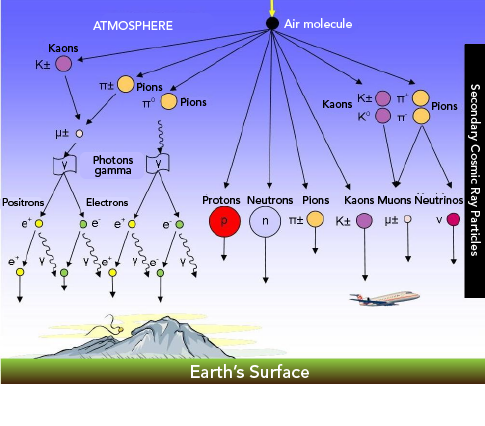
\includegraphics[width=0.7\linewidth]{./fig/Cosmic_ray_scattering.png}
\caption{Cosmic rays and their components. On the left is the soft component, in the middle is the nuclear component and on the right is the hard component \cite{LTSCA}.}
\label{fig:cos}
\end{figure}

\subsection{Nuclear radiation}

As its name implies, nucleons and light atomic nuclei make up nuclear cosmic radiation. Atomic nuclei lose energy through absorption into the air while low energy protons lose theirs through ionization. Neutrons interact abundently with atmospheric nuclei through elastic scattering which creates a gain in thermal energy in said nuclei. The proportion of nuclear radiation reaching the earth's surface is negligible.

\subsection{Soft radiation}

\Pgamma and \Pepm are the constituents of soft cosmic radiation. Electrons arise partially from muon decays but mostly from photon pair creation. Those are mostly produced in two ways: electromagnetic bremsstrahlung/Cherenkov radiation and from the decay of neutral pions \Ppizero. Neutral pions are produced as part of nuclear cosmic radiation and decay into photon pairs with a $8.52 \cdot 10^{-17}\text{ }\si{\second}$ lifetime \cite{Tanabashi:2018oca}. Said photons will overwhelmingly decay into \Pepm pairs if they have an energy $E>2m_{\Pe}$.

\begin{equation*}
\Ppizero\rightarrow\Pgamma\Pgamma,\text{   }\gamma\rightarrow\APelectron\Pelectron,\text{   }\Pepm\rightarrow\Pepm\Pgamma,\text{   }\Pgamma\rightarrow\APelectron\Pelectron \text{   etc.}.
\end{equation*}


The pion's energy will thus be distributed over many particles until a so-called \textit{critical energy} is reached. Under said energy, ionization, as opposed to particle creation, becomes the dominant energy loss mechanism which signals the end of the shower as the number of particles will thus quickly decrease. \Pgamma lose energy through the Compton and photoelectric effects which implies that those remaining particles can easily be shielded by a couple centimetres of lead.

\subsection{Hard radiation}

The hard radiation component is revolves around heavy flavour leptons, mainly \Pmu flavour ones. Due to their relatively high mass, muons only lose small amounts of energy due to bremsstrahlung and mostly through ionization since they have a very high critical energy ($\sim \SI{3.6}{\TeV}$). The energy loss of massive charged particles is described by the \textit{Bethe-Bloch Formula}:

\begin{equation}
-\od{E}{x}=\frac{4\pi n z^2 e^4}{m_{\Pe}}\Big(\text{ln}(\frac{2m_{\Pe}v^2}{I(1-\beta^2)}-\beta^2)  \Big).
\end{equation}

where $E$ is the energy, $x$ the distance, n is the number of electrons per $\text{cm}^3$ in the traversed material, $z \cdot e$ is the electrical charge and $v$ the particle's speed, $I$ is the mean excitation potential of an atom in the material, often approximated by $I\simeq 17.7 Z^{0.85}$ and $\beta$ is the factor $\beta = \frac{v}{c}$. This distribution has its minimum for particles which have a $\beta\gamma \sim 3$ with $\gamma=\frac{1}{\sqrt{1-\beta^2}}$ irrespective of the particle as shown in Figure \ref{fig:BB}. Particle which have such an energy or slightly above it are called \textit{Minimum-Ionizing-Particles} (MIPs).

\begin{figure}[htbp]
\centering
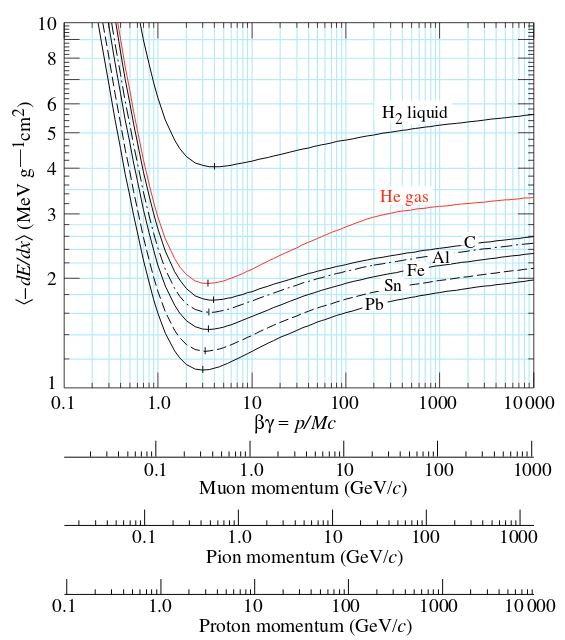
\includegraphics[width=0.7\linewidth]{./fig/BB.png}
\caption{Mean energy loss rate in liquid (bubble chamber) hydrogen, gaseous helium, carbon,aluminum, iron, tin, and lead. Radiative effects, relevant for muons and pions, are not included.These become significant for muons in iron for $\beta\gamma \gtrsim 1000$, and at lower momenta for muons in higher-Z absorbers \cite{Tanabashi:2018oca}.}
\label{fig:BB}
\end{figure}


The energy loss for a MIP in air is $\sim 1.8 \text{ MeV per g/cm}^2$, the number of particles $N$ with energy $E_0$ is given by the integration:

\begin{equation}
N=\int_0^{E_0}\od{E}{E/\text{d}x}.
\end{equation}


When considering the finite number of muons at a given energy and their lifetime of $\tau\sim\SI{2.2}{\micro\second}$, it could be expected that a muon travels a minimum of $\sim \SI{600}{\meter}$ on average in vacuum. If time dilation is accounted for however, the muon's lifetime and thus it's travel distance are increased by a factor $\Pgamma$:

\begin{equation}
\tau_{\Pmu\text{Lab}}=\gamma\tau_{\Pmu}.
\end{equation}

As an example, muons with an energy of \SI{3}{\giga\electronvolt} will have a $\gamma=\frac{E}{m}=\frac{\SI{3}{\giga\electronvolt}}{\SI{105}{\mega\electronvolt}}\sim 29$ leading to a lifetime $\tau \sim \SI{62}{\micro\second}$. It would thus travel $\sim \SI{20}{\kilo\meter}$ in vacuum which corresponds to the approximate height of formation of muons in the atmosphere from pion decays. High-energy muons can make it to the earth's surface almost unhindered and easily pierce through \SI{500}{\meter} of water.

This, in addition to magnetic deflection are the main reasons why the muon momentum-spectrum ($N(E)=\frac{K}{E^{\Pgamma}}$) at ground level is shifted towards high energies as shown in Figure \ref{fig:shift}.

\begin{figure}[htbp]
\centering
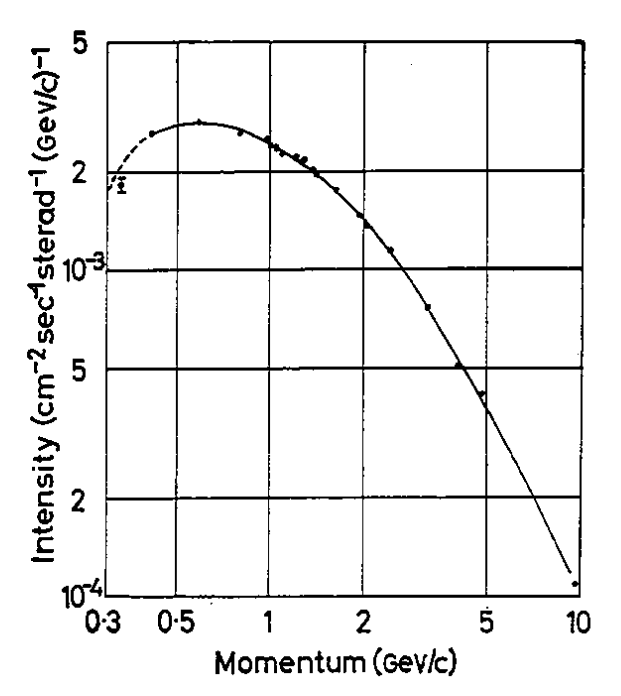
\includegraphics[width=0.5\linewidth]{./fig/shiftDur.png}
\caption{Vertical differential momentum of muons at $54^\circ$ \cite{Gardener_1962}.}
\label{fig:shift}
\end{figure}


\section{Cosmic ray intensity}

In order to perform the experiment, it is necessary to know the width of each cosmic component, especially muons. Table \ref{tab:flx} shows the muon flux as a function of relevant parameters. Figure \ref{fig:cosflux} indicates the flux of various particle productions for different altitudes. At our latitude the muon asymmetry is about 1.3.

\begin{table}
\centering
\tiny
\begin{tabular}{|c|c|c|c|c|c|c|c|c|c|c|c|c|c|}
\hline
\multicolumn{5}{ |c| }{Altitude} & \multicolumn{3}{ |c| }{Total intensity} &\multicolumn{3}{ |c| }{Hard component} &\multicolumn{3}{ |c| }{ Soft Component} \\ \hline
\multicolumn{2}{ |c| }{Distance} & \multicolumn{3}{ |c| }{Pressure} & \makecell{Omni-\\direct-\\ional} & \makecell{Verti-\\cal} & \makecell{Latitude\\effect} & \makecell{Omni-\\direct-\\ional} & \makecell{Verti-\\cal} & \makecell{Latitude\\effect} & \makecell{Omni-\\direct-\\ional} & \makecell{Verti-\\cal} & \makecell{Latitude\\effect} \\ \hline
metres & feet & \si{\milli\meter} Hg & atm & \si{\meter} H$_2$O & \makecell{particle \\ \si{\per sea\cdot\cm\square}} & \makecell{particle \\ \si{\per sea\cdot\cm\square}\\\si{\cdot sterad}} & $\%$ & \makecell{particle \\ \si{\per sea\cdot\cm\square}} & \makecell{particle \\ \si{\per sea\cdot\cm\square}\\\si{\cdot sterad}} & $\%$ &\makecell{particle \\ \si{\per sea\cdot\cm\square}} & \makecell{particle \\ \si{\per sea\cdot\cm\square}\\\si{\cdot sterad}} & $\%$ \\ \hline
0 & 0 & 760 & 1.000 & 10.33 & 0.020 & 0.015 & 10 & 0.013 & 0.000 & 10 & 0.007 & 0.000 & 10 \\
2000 & 6561 & 59.6 & 0.781 & 8.11 & 0.033 & 0.025 & 16 & 0.018 & 0.012 & 15 & 0.017 & 0.013 & 15 \\
4500 & 14764 & 43.3 & 0.870 & 5.59 & 0.10 & 0.07 & 25 & 0.08 & 0.020 & 25 & 0.07 & 0.06 & 25 \\
10000 & 32808 & 10.8 & 0.201 & 2.60 & 0.7 & 0.3 & 45 & 0.10 & 0.05 & 30 & 0.6 & 0.25 & 30 \\
16100 & 52822 & 7.60 & 0.100 & 1.04 & 1.5 & 0.5 & 75 & 0.23 & 0.08 & ? & 1.25 & 0.42 & 80 \\
30000 & 98425 & 0.87 & 0.0115 & 0.118 & 0.5 & 0.15 & 83 & 0.4 & 0.13 & ? & 0.06 & 0.02 & ? \\
$\infty$ & $\infty$ & 0 & 0 & 0 & 0.3 & 0.1 & 00 & ? & ? & ? & ? & ? & ? \\ \hline
\end{tabular}
\caption{Cosmic rays intensity at 50$^\circ$.}
\label{tab:flx}
\end{table}

\begin{figure}[htbp]
\centering
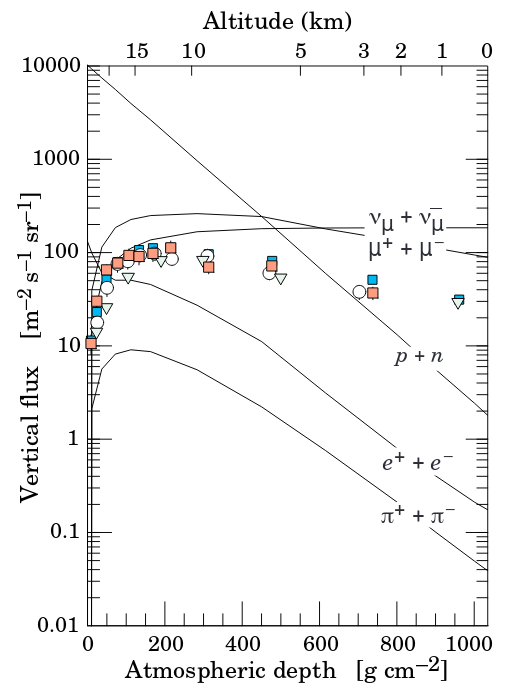
\includegraphics[width=0.5\linewidth]{./fig/cosflux.png}
\caption{Vertical fluxes of cosmic rays in the atmosphere with $E>\SI{1}{\giga\electronvolt}$ estimated from the nucleon flux. The points show measurements of negative muons with $E_{\Pmu} > \SI{1}{\giga\electronvolt}$ \cite{Tanabashi:2018oca}.}
\label{fig:cosflux}
\end{figure}





\bibliography{bib/Experiment41}
\bibliographystyle{abbrv}
\end{document}

